\section{Asynchronous Processing Subsystem}

\subsection{Introduction}

One of Capital Games' primary requirements is to have an asynchronous processing subsystem. This requirement exists both due to the nature of our system, which involves events conditionally occurring at certain time intervals, and the pursuit to build a scalable product. In an attempt to build a system that most closely represents the real stock market, the decision was made to have a pending order queuing system which processes orders at 5 minute intervals. Many orders are processed directly, however some such as short sales and limit orders have conditions associated with them which determine when exactly they are processed. In addition, as the system involves sending summarized reports of player performance metrics at certain time intervals an asynchronous, non-event driven subsystem is highly necessary.\\

\subsection{Nature of the Subsystem}

The asynchronous processing subsystem features three primary components. First, the ability to spawn multiple, independent processes to handle the different kinds of asynchronous tasks. Second, the ability to handle arbitrary object types. And finally, the ability to queue tasks that are waiting to be processed. This is why the Resque Background Process Library built in Ruby was an ideal pick. It allows for the creation of customizable background processes known as "workers". Each worker processes a unique queue. Moreover, each queue can have objects of vastly different types, as long as they implement the function "perform". This is very intuitive as it allows each object to posses the code which acts on it. Lastly, it implements a very smart technique of only storing references to objects in the queue as opposed to the objects themselves so that outdated objects are never processed. This forces the worker to request the most recent version of the object from the DB when it starts being processed. Of course this comes at the slight expense of higher load on the DB when a worker is not sleeping. It is possible that this subsystem will be expanded to incorporate caching techniques. However, they are currently not a requirement. Finally, the queues are stored in RAM for the fastest possible performance. Nevertheless, queues are persisted in JSON encoded flat files to ensure redundancy.\\

\subsection{Structural Model}
The structural model below depicts the overall structure of this subsystem. Namely, the Resque Library and two packages or modules which each are responsible for one kind of task. On the left, the orders package displays a relevant subset of all classes that pertain to placing and processing orders. As previously mentioned, the Order object itself implements the perform method. Therefore, it knows how to process its data when it get gets placed in worker 1's queue. While the OrderHandler class isn't directly involved in the asynchronous processing of orders, it is still relevant in this scope and therefore included in the diagram. It is ultimately the class responsible for placing the order object on the queue when an order is placed. Similarly, the mailer package is depicted with a subset of classes which aggregate data about user performance and send out periodic summarizations of performance metrics to all users on the site. Worker 2 is dedicated to processing email related tasks daily. In this case, the architecture is slightly different as the worker doesn't directly call perform on each ActionMailer object, but instead on a NewsletterController which populates the worker's queue with customized ActionMailer Objects.

\newpage

\subsection{Interaction Diagrams}

There are two interaction diagrams displayed below, each associated with one worker. Due to the inherent background nature of this subsystem, there are relatively few actors involved in this subsystem.\\

\begin{figure}[H]
\centering
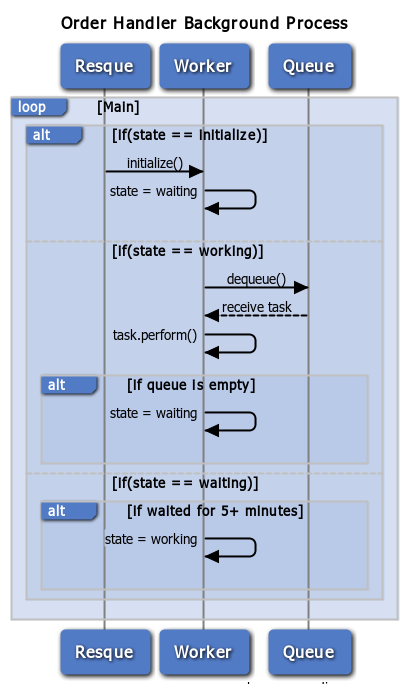
\includegraphics[width=4.5in]{./Diagrams/ComponentModels/stateMachineDiagrams/Worker1/worker1.png}
\caption{The interaction diagram above is roughly divided into two areas, when the process is working and when it is sleeping. This portrays the typical polling behavior of such a background running process. After initialization, when the worker wakes up it attempts to dequeue all objects and call the "perform" method on the object. Since the actual nature of the "perform" method is unique to every object, it is not depicted in this diagram. It is relevant to mention that this individualized execution design allows conditional orders to be processed very easily since the object has all the information needed to make the decision of whether to process at its disposal. Once the queue becomes empty again, the process goes back to sleep. This occurs continually after the spawning of the process.}
\end{figure}

\begin{figure}[H]
\centering
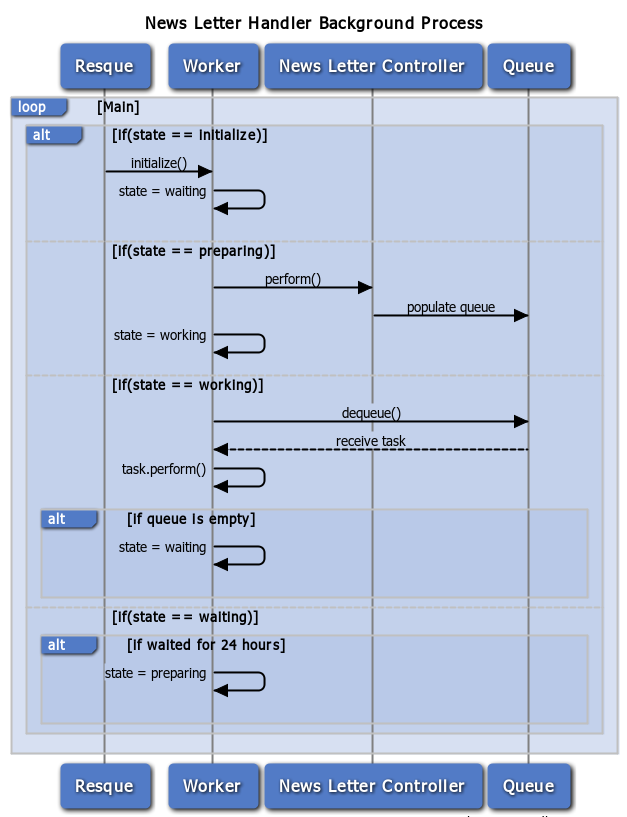
\includegraphics[width=5.5in]{./Diagrams/ComponentModels/stateMachineDiagrams/Worker2/worker2.png}
\caption{Worker 2 behaves a bit differently than worker 1 which results in having an additional state. This "prepare" state is when all the customizing of user-specific emails is done. Afterwards, the process enters the working state where it attempts to fire off all customized emails which were placed onto the queue during the "prepare" state. As in the previous diagram, the diagram incorporates the base case when the worker's queue has been emptied and when the process is sleeping.}
\end{figure}

% Alright, this section requires a solid
% 2-3 pages explaining EVERYTHING LIKE 
% I'M FIVE YEARS OLD. You can't just be like
% "this is how you subsystem". That's what 
% Caggiano does and it's not good enough.
% You need to be like Yates and explain
% everything about the system before you explain
% how to use it. You should explain what a queue
% is, why we chose it (it was the best way to scale
% our load and handle conditional orders), how it's used,
% in what format things are requested and returned
% Then explain how Resque/worker threads abstracts that.
% Then explain the types of methods/classes/jobs you
% created and why they were created. LIKE I'M FIVE!!!
% Then explain how the application interfaces with 
% the subsystem and why I don't need to know your
% subsystem inside and out in order to call into it.
% ONLY THEN can you include diagrams. AND THEN 
% EXPLAIN THEM. People care more about the how and why
% than the what, because from one they should be able
% to intuit the other. 